\documentclass{standalone}
\usepackage{tikz}
\usetikzlibrary{automata,positioning}
\begin{document}
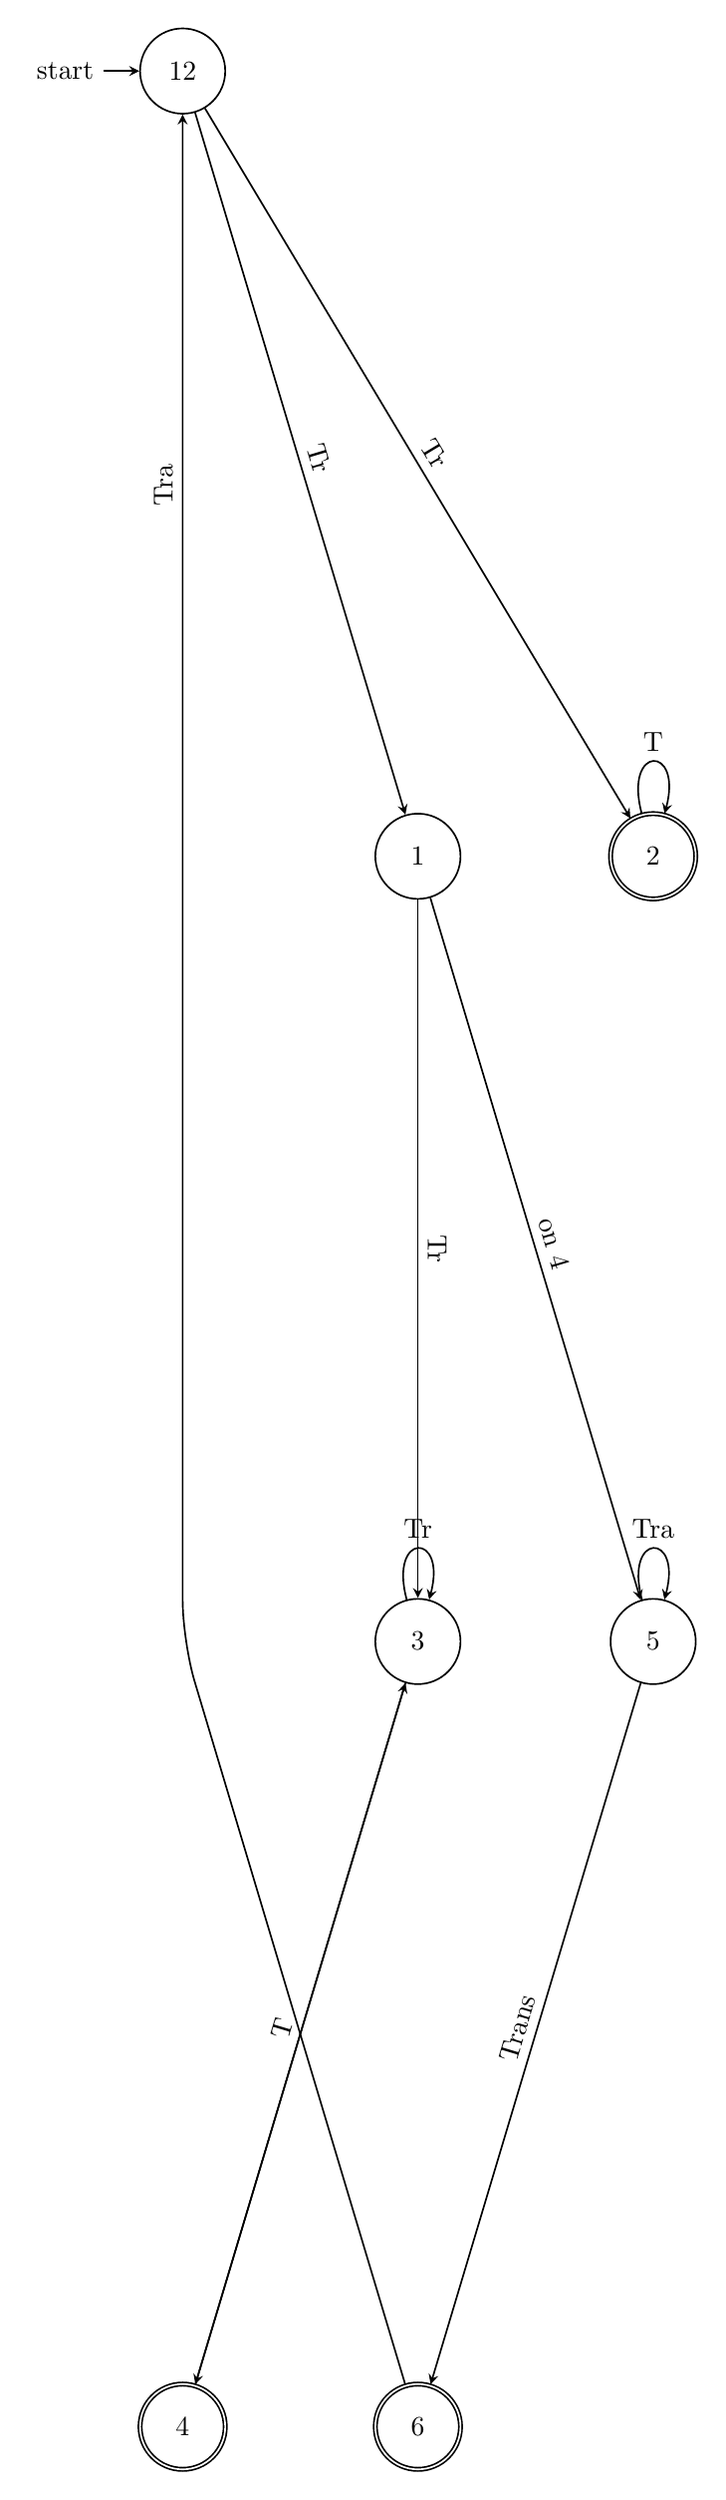
\begin{tikzpicture}[->,>=stealth,auto,node distance=2.5cm,semithick,every state/.style={minimum width=1cm, minimum height=1cm, text width=0.75cm,align=center}]
\node[state, initial] (12) at (0,0) {12};
\node[state] (1) at (3,-10) {1};
\node[state, accepting] (2) at (6,-10) {2};
\node[state] (3) at (3,-20) {3};
\node[state, accepting] (4) at (0,-30) {4};
\node[state] (5) at (6,-20) {5};
\node[state, accepting] (6) at (3,-30) {6};
\draw[->, rounded corners=15pt] (6) -- (0,-20) -- (0,-10) -- (12) node[midway, sloped, above] {Tra};
\path (12) edge node[midway, sloped, above] {Tr} (1);
\path (12) edge node[midway, sloped, above] {Tr} (2);
\path (1) edge node[midway, sloped, above] {Tr} (3);
\path (1) edge node[midway, sloped, above] {on 4} (5);
\path (3) edge node[midway, sloped, above] {T} (4);
\path (4) edge node[midway, sloped, above] {} (3);
\path (5) edge node[midway, sloped, above] {Trans} (6);
\draw[->, loop above] (2) to node[sloped, above] {T} (2);
\draw[->, loop above] (3) to node[sloped, above] {Tr} (3);
\draw[->, loop above] (5) to node[sloped, above] {Tra} (5);
\end{tikzpicture}
\end{document}